\chapter{Technologie Evaluation}
In diesem Kapitel werden relevante Technologien und Frameworks, welche das Front-End, Back-End, sowie die Datenbank betreffen, evaluiert. Für jeden dieser Bereiche wurden Kriterien erarbeitet. Die Auswahl geschieht aufgrund der Bewertung anhand dieser Kriterien.

\section{Back-End}
Die Entscheidung des Frameworks für das Back-End ist von grosser Tragweite. Heutzutage existieren einige beliebte Frameworks um Web Applikationen zu erstellen. Die zu verwendende Programmiersprache ist bei vielen Frameworks ebenfalls unterschiedlich und sollte berücksichtigt werden.

\subsection{Kriterien}
\begin{itemize}
\item Open-Source
\item Gute Dokumentation und Unterstützung durch die Community
\item Einfache Bedienung und schnelle Einarbeitung
\item Performance / Skalierbarkeit
\item Libraries für IoT-Kommunikationsprotokolle
\item Kenntnisse der Programmiersprache
\end{itemize}

\begin{longtable}{| p{4cm} | p{11.7cm} |}
\hline
\textbf{Node.js}\newline
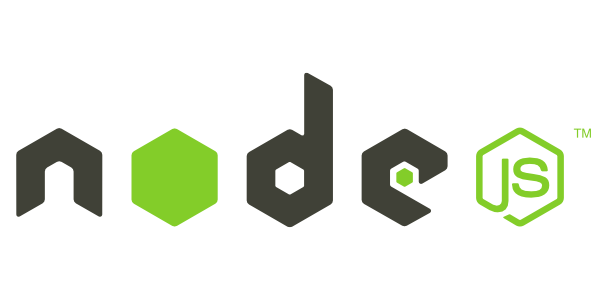
\includegraphics[width=0.25\columnwidth]{../03_Design/images/nodejs_logo.png} & Node.js ist eine Plattform für serverseitiges JavaScript. Das I/O-Handling ist event-driven und nicht-blockierend. Jeder Node.js Prozess ist single-threaded. Node.js hat viele Erweiterungsmodule wie z.B. Express um Web Applikationen zu erstellen. Für Web Applikationen ist Node.js mit Express besonders gut geeignet, da auf Client- und Serverseite mit JavaScript gearbeitet werden kann. Die Anzahl möglicher Verbindungen könnten trotz Single-Threading gut verarbeitet werden da die Anfragen asynchron mit einem Callback an die Devices gesendet werden, der aktive Thread würde somit nicht blockieren.
\newline
\newline
\textbf{Vorteile} \newline
\tabitem Einfacher Einstieg \newline
\tabitem Weite Verbreitung und gute Community-Unterstützung \newline
\tabitem Gute Skalierbarkeit (non-blocking) \newline
\tabitem Grundkenntnisse beim Entwicklerteam vorhanden \newline
\tabitem Gleiche Programmiersprache beim Front- und Backen \newline
\textbf{Nachteile} \newline
\tabitem Kein Multi-Threading \newline
\tabitem Interpretierte Skriptsprache \newline
\tabitem Schwache Objektorientierung (kein Polymorphismus, Duck-Typing, etc.)\\ \hline
\textbf{Spring MVC}\newline

\includegraphics[width=0.25\columnwidth]{../03_Design/images/spring_logo.png}
& Spring MVC wird verwendet um dynamische Webseiten mit Java Servlets zu erstellen. Dependency Injection und aspektorientierte Programmierung sind ebenfalls unterstützt. Konfigurationen über XML und Java Annotations unterstützen den Entwickler beim Erstellen von MVC Web-Applikationen. Die Library-Unterstützung für IoT-spezifische Kommunikationsprotokolle wie beispielsweise CoAP sind bei Java EE hervorragend. Java unterstützt sowohl Multi-Threading, als auch non-blocking I/O. Gleichzeitige Verbindungen zu Devices könnten in eigene Threads ausgelagert werden, um nicht das gesamte Back-End zu blockieren.
\newline
\newline
\textbf{Vorteile} \newline
\tabitem Weite Verbreitung und gute Community-Unterstützung \newline
\tabitem Gute Skalierbarkeit (Multi-Threading) \newline
\tabitem Gute Java Programmierkenntnisse beim Entwicklerteam vorhanden \newline
\tabitem Kompilierte Sprache \newline
\tabitem Starke Objektorientierung (Polymorphismus, Type-Safety, etc.) \newline
\tabitem Dependency-Injection Unterstützung \newline
\textbf{Nachteile} \newline
\tabitem Umgang mit Spring MVC müsste vom Entwicklerteam erlernt werden \newline
\tabitem Unterschiedliche Sprachen für Front- und Back-End
\\ \hline 
\end{longtable}

\subsection{Skalierbarkeit}
Da potenziell viele Devices über die Applikation verwaltet werden könnten ist die Skalierbarkeit von grosser Bedeutung. Die Art der Verbindungen unterscheiden sich. Während die Anzahl gleichzeitiger Verbindungen über das Front-End zum Server (concurrent users) sehr gering sein wird, besteht die Möglichkeit, dass hunderte oder gar tausende IoT-Devices verbunden sind.

Es besteht jedoch nicht die Notwendigkeit, dass während der Nutzungsdauer alle diese Verbindungen aufgebaut und offen gehalten werden. Es ist damit zu rechnen, dass niemals mehr als 100 gleichzeitige Verbindungen zu unterschiedlichen Devices existieren. 

\subsection{Entscheidung}
Die Entscheidung fiel auf Spring MVC. Eine Implementation mittels Node.js und Express wäre ebenfalls denkbar, da alle Anforderungen und Restriktionen erfüllt werden könnten. Auch andere Frameworks wie Django oder Ruby on Rails würden ebenfalls in Frage kommen, wurden aber nicht berücksichtigt da keine oder nur kaum Vorkenntnisse beim Entwicklerteam vorhanden waren.

Ausschlaggebend für die Auswahl von Spring MVC ist die zugrundeliegende Programmiersprache Java. Die Unterstützung von Klassen, Vererbung und Polymorphie sowie die grosse Unterstützung von Tools und Plugins ermöglichen eine angenehmere und übersichtlichere Entwicklung. Durch die Unterstützung mittels XML Konfigurationen und Java Annotations werden die Entwickler mit Spring MVC hervorragend unterstützt.

\newpage
\section{Front-End}
Das Front-End der Applikation muss dem Benutzer auf eine einfache und übersichtliche Weise die Interaktion ermöglichen. Es sollen einerseits neue Geräte hinzugefügt werden, andererseits bestehende Geräte verwaltet oder überwacht werden. Potenziell könnten eine grosse Anzahl solcher IoT-Devices vorliegen, weshalb diese übersichtlich gruppiert werden sollen.

\subsection{Kriterien}
\begin{itemize}
\item Webbasierter Zugriff
\item Responsive Web Design für unterschiedliche Bildschirmgrössen
\item Einfache Bedienung und schnelle Einarbeitung
\item Gute Dokumentation und Unterstützung durch die Community
\end{itemize}

\subsection{Varianten}
Bei der Variantenauswahl wurden drei sich stark unterscheidende Ansätze gewählt. Grundsätzlich wären weitere Frameworkalternativen zu Bootstrap und Angular.js denkbar.

\begin{longtable}{| p{4cm} | p{11.7cm} |}
 \hline
  \textbf{Hardcoding} & Hardcoding des Frontends bringt wenige Vorteile. Sämtlicher HTML, CSS und JavaScript Code müsste von Hand geschrieben werden. Ein selber erstelltes responsives Layout mit CSS ist zwar möglich, aber aufwändig. Es müsste somit viel Zeit in das Layout und das Styling für ein ansprechendes Ergebnis investiert werden. Eine Cross-Browser Unterstützung ist ebenfalls schwierig.\\ \hline 
 \textbf{Twitter Bootstrap} & Bootstrap von Twitter ist ein weit verbreitetes Framework für Webseiten. Responsive Layouts für unterschiedliche Bildschirmgrössen werden unterstützt. Elemente wie Buttons, Drop-Down Menüs und ähnliches werden von Bootstrap auf sehr einfache Weise bereitgestellt. Die JavaScript Funktionalitäten beschränken sich auf die Anzeige von UI Elementen. Falls JavaScript für die Programmierung der Applikation verwendet wird sollte ein weiteres Framework dafür verwendet werden.\\ \hline 
 \textbf{Angular.js} & Angular.js ist ein bekanntes Framework für Single Page Applications (SPA) im MVC Stil. Angular.js ist TypeScript 2 basiert, hat Dependency Injection Mechanismen eingebaut, unterstützt 2-way Databinding und Unit Testing. Die Software Architektur ist Client-konzentriert, MVC passiert im Browser.\\ \hline
\end{longtable}

\subsection{Entscheidung}
Durch die einfache und schnelle Entwicklungsmöglichkeiten wurde Bootstrap gewählt. Angular.js hat klare Vorteile bei der Erstellung von Single Page Applications. Nach jetztigen Erkenntnissen sind jedoch keine aufwändigen Funktionen clientseitig vorgesehen, Data-Binding scheint zum heutigen Zeitpunkt nicht notwendig. 

Dem Projektteam ist Angular.js unbekannt und es müsste mit einer langen Einarbeitungszeit und anfänglich schlechter Code-Qualität gerechnet werden. Falls zu einem späteren Zeitpunkt weitere Anforderungen und Funktionen vorgesehen werden, wäre eine \glqq echte\grqq  Single Page Application mit Angular.js eine echte Alternative und könnte die \glqq einfache\grqq Variante mit Bootstrap von Twitter ergänzen oder ablösen.

\newpage
\section{Datenbanktechnologie}
Für die Persistierung der Objekte stehen zwei grundlegende Verfahren zur Verfügung. SQL (Structured Query Language) war über einen langen Zeitraum die Standardtechnologie für die Persistierung von Datenobjekten, mit NoSQL Technologien ist jedoch eine starke Alternative mit einigen Vorteilen gegenüber der herkömmlichen SQL Technologie entstanden.

\subsection{SQL}
SQL basiert auf einem relationalen Datenmodell. Die Objeke werden auf Tabellen abgebildet. Eine Tabelle stellt somit ein Typ- und die Columns Felder dar. Mit SQL-Datenbanken wird ein stark normalisiertes Datenmodell ohne Redundanzen angestrebt. Mittels referenzieller Integrität (Fremdschlüsselwerte in Tabelle X müssen als Primärschlüsselwerte in Tabelle Y vorhanden sein) wird eine starke Datenkonsistenz gewährleistet. Ein Datensatz kann daher nur gelöscht werden, wenn keine Referenzen darauf zeigen. Mittels Joins von Tabellen können zusammenhängende Datensätze mit einem einzelnen Query abgefragt werden.

Ein grosser Nachteil bei SQL ist das strikte Datenschema. Die Tabelle gibt genau vor, welche Columns für das Objekt existieren (müssen). Möchte man weitere Werte respektive Columns hinzufügen, so müsste das gesamte Schema der Tabelle angepasst werden (altering).

\subsection{NoSQL}
Mit NoSQL werden die Daten als Key-Value Paare in einem strukturierten Format gespeichert. Häufig ist dies JSON (JavaScript Object Notation). Eine Collection steht für einen Typ von Daten und enthält entweder Key-Value Paare oder weitere Collections. Beziehungen zu anderen Objekten können auf zwei verschiedene Arten erfolgen; entweder als embedded Collection (Denormalisierung) oder mittels Referenz auf ein anderes Objekt.

Ein grosser Vorteil ist das flexible Datenmodell. Wenn man sich beispielsweise ein persistiertes Device-Objekt anschaut, so könnte dies wie folgt aussehen:
\begin{lstlisting}[language=json]
{
    "_id":{
        "id": "58ecfe09beedc31188fc0281",
        "name":  "Device XY",
        "protocolType": "HTTP",
        "authType": "BASIC_AUTH",
        "endpoint": "http://some.domain.com/path",
        "username": "admin",
        "password": "1234"
        }    
}
\end{lstlisting}
Falls ein weiteres Attribut gespeichert werden müsste, ist dies bei NoSQL nicht weiter problematisch. Die Datenbank speichert die Objekte auch mit anderen Attributen resp. Key-Value Paaren.

\newpage
NoSQL selbst unterteilt sich in verschiedene Datenmodelle. \cite{WikiNoSQL}
\begin{longtable}{| p{4cm} | p{11.7cm} |}
\hline
\textbf{Key-Value} & Leistung: hoch \newline Skalierbarkeit: hoch \newline Flexibilität: hoch \newline Komplexität: keine \newline Funktionalität: keine \newline
Durch die Einfachheit des zugrunde liegenden Datenmodells lassen sich Datensätze schnell (in O(1)) abfragen. Komplexere Abfragen über Verknüpfung der Objekte sind deutlich langsamer. Bei einer hohen Frequenz von Abfragen und Speicherung von Key-Value Tupeln ist diese Form von Datenbank geeignet.
\\ \hline
\textbf{Spaltenorientiert} & Leistung: hoch \newline Skalierbarkeit: hoch \newline Flexibilität: mittel \newline Komplexität: gering \newline Funktionalität: minimal \newline
Das zugrunde liegende Datenmodell basiert auf der Speicherung der Spaltenwerte. Während normalerweise Datensätze auf einer Zeile mit ihren unterschiedlichen Spalten abgelegt werden, so wird bei dieser Art zuerst eine komplette Spalte gespeichert bevor mit Werten aus einer anderen Spalte forgefahren wird. 
\\ \hline
\textbf{Dokumentenorientiert} & Leistung: hoch \newline Skalierbarkeit: hoch \newline Flexibilität: hoch \newline Komplexität: gering \newline Funktionalität: gering \newline
Dokumente bilden das Schema einer Entität. Eine dokumentenbasierte Datenbank kann mehrere solcher Dokumente enthalten. Dokumente sind quasi das Gegenstück zu Tabellen in einer relationalen Datenbank. Ein Dokument liegt meist im JSON Format vor und hält seine Objekte eingebettet. 
\\ \hline
\textbf{Graphbasiert} & Leistung: unterschiedlich \newline Skalierbarkeit: unterschiedlich \newline Flexibilität: hoch \newline Komplexität: hoch \newline Funktionalität: gem. Graphentheorie \newline
Eine Graphendatenbank speichert Knoten und Kanten. Knoten sind Entitäten und Kanten deren Beziehungen. Dieses Datenmodell eignet sich für die Modellierung und Speicherung von Netzwerken wie beispielsweise Social Media.
\\ \hline
\end{longtable}
 \newpage

\subsection{Entscheidung}
NoSQL wurde als geeignetere Variante für die Speicherung der Objekte ausgewählt. Bei vielen unterschiedlichen Devicetypen muss davon ausgegangen werden, dass Änderungen respektive Ungleichheiten am Schema auftauchen werden. Ein starres, relationales Modell würde dies stark erschweren, da jedes mal mittels \glqq ALTER TABLE\grqq  das Schema geändert- und bestehende Datensätze angepasst werden müssten.

Als NoSQL Implementation wurde \glqq mongoDB\grqq ausgewählt. MongoDB ist eine dokumentenorientierte Datenbank, welche Objekte im BSON Format abspeichert. Die Entitäten werden in sogenannten \glqq Collections\grqq  abgelegt. Attribute der Collections können einzeln abgefragt werden. Die Struktur der Collections ist flexibel, Attribute von Objekten innerhalb der Collections dürfen sich unterscheiden. MongoDB ist die zurzeit wohl am weitest verbreitete NoSQL Implementation, weshalb eine grosse Community und umfangreiche Online-Hilfen verfügbar sind.
 




